% Basic info about your document: a4 paper, 11pt font size, article style.
\documentclass[a4paper, 11pt]{article}

\usepackage{graphicx} % Enables adding figures
\usepackage[a4paper, margin=18mm]{geometry} % Let's you adjust the margins
\usepackage[T1]{fontenc} % Font helvetica
\usepackage[scaled]{helvet}
\usepackage{authblk} % multiauthor
\usepackage{multirow} % table
\usepackage[table,xcdraw]{xcolor}
\usepackage{float} % position des figures,table
\usepackage[backend=biber,style=numeric,sorting=none]{biblatex} % bibliographie
\usepackage{fancyhdr} % footer
\usepackage{caption} % caption
\usepackage{multicol} % multicolonne

%Setup bibliographie
\addbibresource{bibliographie.bib} % utilise bibliographie.bib pour la bibliographie

%Setup figure
\graphicspath{ {./figure/} } % relative path for figure

\renewcommand\familydefault{\sfdefault} % set font for all document
\captionsetup[table]{name=Tableau} % Rename table
\renewcommand*\contentsname{Table des matières} % Rename table of contents
\setlength\parindent{0pt} % remove indent in new line

%Setup Titre, auteur et date
\title{
    \vspace{-2.5cm}
    \centering\includegraphics[scale=0.5]{Logos\_Hepia.png}\\
    \centering\rule{17cm}{0.1mm}\vspace*{0.4in}\\
    \centering Projet thématique MOON}
\renewcommand\Authands{ et } % replace "and" by "et" in author
\author[1]{AYRINHAC Elisa}
\author[2]{DROUIN Clément}
\author[3]{JOUCLARD Charly}
\affil[1]{HEPIA, MT2, elisa.ayrinhac@hes-so.ch}
\affil[2]{HEPIA, MT2, clement.drouin@hes-so.ch}
\affil[3]{HEPIA, MT2, charly.jouclard@hes-so.ch}
\date{28 avril 2023}

%Setup header, footer
\pagestyle{fancy}
\fancyhead{} % clear all header fields
\renewcommand{\headrulewidth}{0pt} % no line in header area
\fancyfoot{} % clear all footer fields
\renewcommand{\footrulewidth}{1pt}
\newcommand{\changefont}{\fontsize{9}{11}\selectfont}
\newcommand{\TheAuthor}{AYRINHAC Elisa, DROUIN Clément, JOUCLARD Charly}
\fancyfoot[C]{\changefont\TheAuthor}
\fancyfoot[R]{\changefont\thepage}
\fancyfoot[L]{\changefont Projet thématique MOON}

\begin{document}

%Entete
\maketitle
\thispagestyle{empty}
\begin{center}
    \rule{\textwidth}{0.1mm}
\end{center}
%Introduction
\vspace{-1cm}
\section*{Introduction}
Le projet thématique vient se placer dans le cadre des études de bachelor en microtechnique, option Bio-ingénierie. Cette année, le projet porte sur l'endométriose, une maladie encore peu connue touchant 1 femme sur 10.\\
Les objectifs du projet sont, d'une part, de mettre en application les connaissances acquises durant nos études, mais également de développer de nouvelles compétences comme la gestion de projet.
D'autre part, ce projet contribue à développer la recherche sur l'endométriose et servira de support pour le \\
"project MOON : endoMetriosis Organoids to vOice up woman paiN".\\
Le but est donc de créer un bio-chip qui permettrait d'étudier les tissus de l'endomètre soumis à différentes concentrations d'hormones.
\newpage
%Table des matieres
\tableofcontents
\newpage
%Debut rapport
\section{Etudes préliminaire}
\subsection{Biologie}
Afin de mieux comprendre comment concevoir un appareil correspondant à la demande du client, une courte introduction biologique est nécessaire.\\
L'endométriose se caractérise par le développement d'un tissu semblable à l'endomètre en dehors de l'utérus. Généralement, le tissu endométrial se développe dans les ovaires, et il peut former des kystes remplis de sang appelés endométriomes. Ces kystes peuvent varier en taille et provoquer des symptômes qui varient énormément entre les femmes, mais on retient le plus souvent celui de la douleur extrême.\\
Cependant, il est également possible que des lésions similaires à des kystes endométriomes apparaissent sur les organes pelviens adjacents aux ovaires tels que les trompes de Fallope, les ligaments utéro-sacrés, la vessie, etc.\\
L'endomètre est un épithélium qui compose une partie de l'appareil reproducteur féminin. Il tapisse les parois de la cavité utérine et est composé de 3 couches : le myomètre qui est la fondation de l'endomètre, la couche basale qui contient les glandes et les tissus conjonctifs, et la couche fonctionnelle.\\
Cette dernière couche est celle qui voit sa taille changer durant le cycle menstruel, qui est régulé par 4 hormones.
\subsection{Etat de l'art}
Actuellement la culture cellulaire est un procédé connu et maitriser par l'Homme qui consiste à placer des cellules dans un milieu de culture afin de les faire proliférer.
Cette méthode permet d'avoir des colonies de cellule pouvant aller jusqu'a formé des organoïdes.
Organoïdes pouvant être utilisés à des fins de recherche sur l'organe miniaturisé.
La méthode d'incubation consiste à placer dans un incubateur une colonie de cellules contenue dans un milieu nutritif.
Pour maintenir de bonnes conditions on place ces échantillons dans l'enceinte d'un incubateur qui permet d'isoler les cellules du milieu extérieur tout en maintenant les constantes de températures, d'humidité et de CO2 de façon optimal.
Les incubateurs professionnels sont des machines de précision, asservis qui permettent de réglée précisément toutes les conditions de leurs enceinte, cela permet de chercher l'expression de certain phénotype au seins des colonies.
Ils sont aussi dotés de sécurité notamment en termes de ventilation afin de protège les cellules et le biologiste. Toutefois cette précision rend le matériel chère.
Il faut compter entre 5000CHF et 15000 CHF pour un incubateur professionnel.
L'incubateur fait maison sont moins précis mais permette une personnalisation complète en termes de condition de culture.
Toutefois même si cela reste compliqué à construire dans sa totalité, il est assez simple de stabiliser la température et l'humidité.
Ces machines permettent de crée une atmosphère apte à la reproduction cellulaire toutefois afin de contenir les cellules et leurs milieu nutritif il faut des instruments de culture.
L'écouvillons : Il s'agit de petit tube munis d'un couvercle étanche en plastique dans lequel on place un peu de liquide du fait de leurs petite taille et de leurs facilités de conception ils peuvent être alignés afin de facilité la reproductivité toutefois il ne possède aucune capacité permettant de maintenir l'homéostasie de la cellule.
La verrerie de chimie : On peut utiliser techniquement tout contenant biocompatible.
\newpage
\subsection{Aperçu du projet}
\subsubsection{Besoins}
On peut voir avec la figure \ref{fig:bete_corne} que le système conçu va permettre au biologiste d'étudier l'influence des hormones sur du tissus endométrial.
\begin{figure}[H]
    \centering
    \resizebox{\linewidth}{!}{\includegraphics{bete\_corne.png}}
    \caption{Bête à corne}
    \label{fig:bete_corne}
\end{figure}
\subsubsection{Fonctions}
\begin{table}[H]
    \centering
    \begin{tabular}{|
            >{\columncolor[HTML]{CBCEFB}}l |l|}
        \hline
        \multicolumn{1}{|c|}{\cellcolor[HTML]{CBCEFB}\textbf{N°}} & \textbf{Fonction}                                 \\ \hline
        FP1                                                       & Maintenir les cellules en vie                     \\ \hline
        FP2                                                       & Intégrer des concentrations spécifiques d'hormone \\ \hline
        FC3                                                       & Observer les cellules au microscope               \\ \hline
        FC4                                                       & Alimenter le système en énergie                   \\ \hline
        FC5                                                       & Réaliser un système autonome                      \\ \hline
        FC6                                                       & Résister au milieu imposer par les cellules       \\ \hline
        FC7                                                       & Utiliser un matériau biocompatible                \\ \hline
        FC8                                                       & Respecter le budget                               \\ \hline
        FC9                                                       & Assurer un cycle de 28 jours                      \\ \hline
    \end{tabular}
    \caption{Fonctions à assurer}
\end{table}
\begin{figure}[H]
    \centering
    \resizebox{\linewidth}{!}{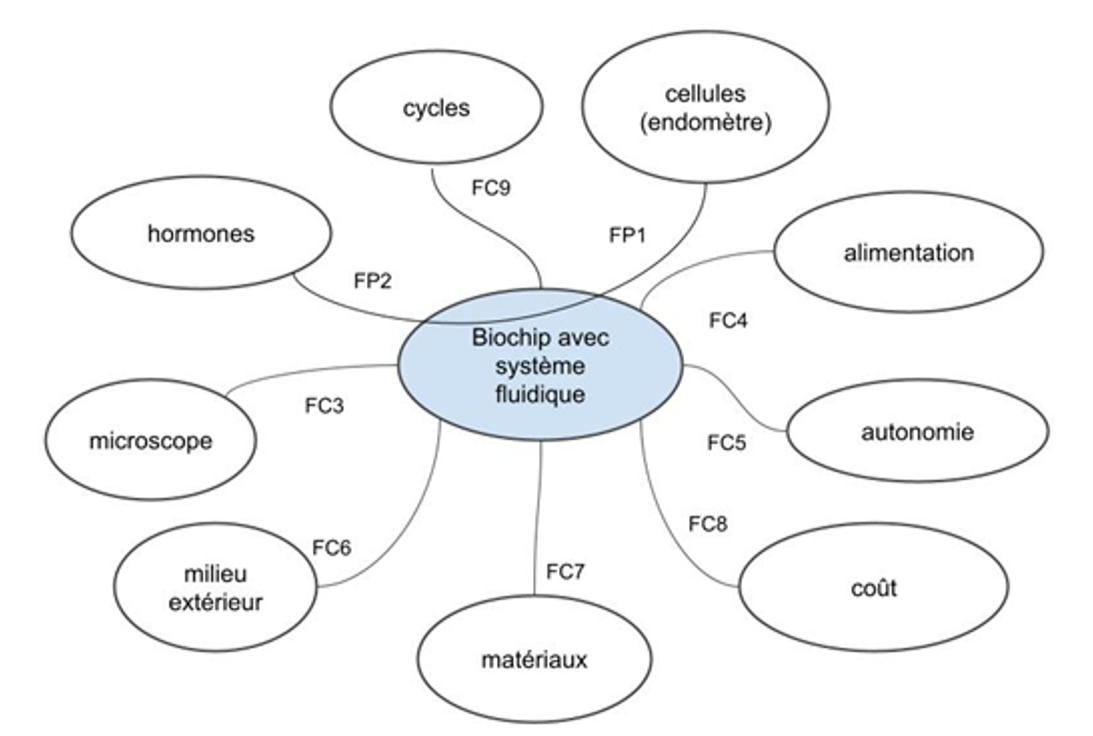
\includegraphics{pieuvre.png}}
    \caption{Diagramme pieuvre avec les fonctions associés}
    \label{fig:pieuvre}
\end{figure}
\subsection{Cahier des charges}
La première fonction à prendre en compte est la survie des cellules.
Pour cela, notre système devra respecter les paramètres suivants :
\begin{itemize}
    \item une température de 37°C
    \item un pH de 7
    \item un renouvellement du milieu de culture de 1 ml par jours
    \item atténué toute variation de milieu
    \item la Biocompatibilité du milieu
\end{itemize}
Pour ce qui est du système fluidique, il permet l'apport du milieu de culture à la cellule et donc nécessite de répondre aux points suivants :
\begin{itemize}
    \item un système étanche
    \item un écoulement laminaire
    \item un système de purge
    \item un système d'injection d'hormones
    \item un mélangeur pour éviter des pics de concentration
    \item une pompe pour un système dynamique
\end{itemize}
Enfin, le système dans sa globalité devra assurer :
\begin{itemize}
    \item une autonomie de 28 jours minimum
    \item une zone transparente permettant l'observation des cellules
\end{itemize}
\subsection{Catalogue de solutions}
\subsubsection{Gestion des nutriments, déchets et de la concentration des hormones}
\begin{table}[H]
    \centering
    \begin{tabular}{|l|l|l|}
        \hline
        \multicolumn{1}{|c|}{\textbf{Solution}}        & \textbf{Avantages}                                                                                                     & \textbf{Inconvénients}                                                                                                             \\ \hline
        Seringues auto-poussés                         & \begin{tabular}[c]{@{}l@{}}-Précis\\ -Facile d'utilisation\\ -Facilement programmable\\ -Réponse linéaire\end{tabular} & \begin{tabular}[c]{@{}l@{}}-Energie\\ -Limité en quantité\\ -Espace\end{tabular}                                                   \\ \hline
        \rowcolor[HTML]{CBCEFB}
        Pompe péristaltiques\cite{pompe_peristaltique} & -Déjà présent au labo                                                                                                  & \begin{tabular}[c]{@{}l@{}}-Peu précis\\ -Energie\end{tabular}                                                                     \\ \hline
        Système de goutte à goutte                     & \begin{tabular}[c]{@{}l@{}}-Low-cost\\ -Economique en énergie\end{tabular}                                             & \begin{tabular}[c]{@{}l@{}}-Précision\\ -A pression atmosphérique\\ -Complexité d'asservissement\\ -Réponse chaotique\end{tabular} \\ \hline
    \end{tabular}
    \caption{Solutions pour la gestions des nutriments, déchets et des hormones}
\end{table}
\subsubsection{Contrôler l'environnement extérieur}
\begin{table}[H]
    \centering
    \begin{tabular}{|l|l|l|}
        \hline
        \multicolumn{1}{|c|}{\textbf{Solution}} & \textbf{Avantages}                                                                                        & \textbf{Inconvénients}                                                                      \\ \hline
        \rowcolor[HTML]{CBCEFB}
        Incubateur                              & \begin{tabular}[c]{@{}l@{}}-Constante externe stable\\ -A disposition\\ -Retour d'expérience\end{tabular} & \begin{tabular}[c]{@{}l@{}}-Placé dans l'incubateur\\ -Protéger l'électronique\end{tabular} \\ \hline
        Système autonome                        & -Pas de dépendance                                                                                        & \begin{tabular}[c]{@{}l@{}}-Compliqué à réaliser\\ -Energivore\\ -Coût\end{tabular}         \\ \hline
    \end{tabular}
    \caption{Solutions pour gérer l'environnement extérieur}
\end{table}
\subsubsection{Cultiver les cellules}
\begin{table}[H]
    \centering
    \begin{tabular}{|l|l|l|}
        \hline
        \multicolumn{1}{|c|}{\textbf{Solution}} & \textbf{Avantages}                                                                                         & \textbf{Inconvénients}                                                             \\ \hline
        \rowcolor[HTML]{CBCEFB}
        Bio-chip en PMMA                        & \begin{tabular}[c]{@{}l@{}}-Usinage\\ -Retour d'expérience\\ -Sur mesure\\ -Fluidique intégré\end{tabular} & \begin{tabular}[c]{@{}l@{}}-Assemblage par couche\\ -Long à fabriquer\end{tabular} \\ \hline
        Boîte de pétris                         & \begin{tabular}[c]{@{}l@{}}-Coût\\ -Stérilité\end{tabular}                                                 & -Pas de circulation de fluide                                                      \\ \hline
    \end{tabular}
    \caption{Solutions pour le milieu de culture}
\end{table}
\subsubsection{Circulation du fluide}
\begin{table}[H]
    \centering
    \begin{tabular}{|l|l|l|}
        \hline
        \multicolumn{1}{|c|}{\textbf{Solution}} & \textbf{Avantages}                                                                                            & \textbf{Inconvénients}                                           \\ \hline
        \rowcolor[HTML]{CBCEFB}
        Pompe péristaltique                     & \begin{tabular}[c]{@{}l@{}}-Déjà présent au labo\\ -Facile d'utilisation\\ -Pas de contamination\end{tabular} & \begin{tabular}[c]{@{}l@{}}-Débit limité\\ -Energie\end{tabular} \\ \hline
        Gravité                                 & \begin{tabular}[c]{@{}l@{}}-Pas besoin de matériel spécifique\\ -Pas besoin d'alimentation\end{tabular}       & -Compliqué à mettre en oeuvre                                    \\ \hline
    \end{tabular}
    \caption{Solutions pour injecter les différents fluides}
\end{table}
\subsubsection{Mélanger les fluides}
\begin{table}[H]
    \centering
    \begin{tabular}{|l|l|l|}
        \hline
        \multicolumn{1}{|c|}{\textbf{Solution}} & \textbf{Avantages}                                                                                                           & \textbf{Inconvénients}                                                                                  \\ \hline
        \rowcolor[HTML]{CBCEFB}
        Mélangeur hydrostatique "2D"            & \begin{tabular}[c]{@{}l@{}}-Economique\\ -Facilité d'intégration\\ -Compact\\ -Volume sur mesure\\ -Modélisable\end{tabular} & \begin{tabular}[c]{@{}l@{}}-A créer\\ -Perte de charge\end{tabular}                                     \\ \hline
        Mélangeur hydrostatique "3D"            & \begin{tabular}[c]{@{}l@{}}-Economique\\ -Facilité d'intégration\\ -Compact\\ -Volume sur mesure\\ -Modélisable\end{tabular} & \begin{tabular}[c]{@{}l@{}}-A créer\\ -Perte de charge\\ -Usinage\end{tabular}                          \\ \hline
        Mélangeur magnétique                    & \begin{tabular}[c]{@{}l@{}}-Déjà présent au labo\\ -Facilement nettoyable\\ -Gestion de la puissance\end{tabular}            & \begin{tabular}[c]{@{}l@{}}-Espace\\ -Biocompatibilité\\ -Non modélisable\\ -Non pilotable\end{tabular} \\ \hline
    \end{tabular}
    \caption{Solutions pour assurer l'homogénéité des liquides}
\end{table}
\subsubsection{Analyser les concentrations}
\begin{table}[H]
    \centering
    \begin{tabular}{|l|l|l|}
        \hline
        \multicolumn{1}{|c|}{\textbf{Solution}} & \textbf{Avantages}                                                                                                                  & \textbf{Inconvénients}                                                                           \\ \hline
        \rowcolor[HTML]{CBCEFB}
        Colorimètre externe                     & \begin{tabular}[c]{@{}l@{}}-Facilité d'intégration\\ -Précis\\ -Déjà présent au labo\end{tabular}                                   & \begin{tabular}[c]{@{}l@{}}-Aucune donnée interne\\ -Nécessite présence utilisateur\end{tabular} \\ \hline
        Colorimètre interne                     & \begin{tabular}[c]{@{}l@{}}-Retour en temps réel\\ -Gain de précision de l'asservissement\\ -Donnée interne au système\end{tabular} & \begin{tabular}[c]{@{}l@{}}-A créer\\ -Précision\end{tabular}                                    \\ \hline
    \end{tabular}
    \caption{Solutions pour contrôler les concentrations}
\end{table}
\subsubsection{Contrôler le système (microcontrôleur)}
\begin{table}[H]
    \centering
    \begin{tabular}{|l|l|l|}
        \hline
        \multicolumn{1}{|c|}{\textbf{Solution}} & \textbf{Avantages}                                                                                                                                      & \textbf{Inconvénients}                                                                                                                           \\ \hline
        Arduino Uno                             & \begin{tabular}[c]{@{}l@{}}-Facilité d'utilisation\\ -Flexible\end{tabular}                                                                             & \begin{tabular}[c]{@{}l@{}}-Pas de stockage interne\\ -Pas de contrôle à distance\\ -Pas de possibilité d'utiliser python\\ -14 pin\end{tabular} \\ \hline
        \rowcolor[HTML]{CBCEFB}
        Raspberry Pi                            & \begin{tabular}[c]{@{}l@{}}-Retour en temps réel\\ -Contrôlable à distance\\ -Stockage interne\\ -Utilisation possible de Python\\ -40 pin\end{tabular} & -Faible disponibilité                                                                                                                            \\ \hline
    \end{tabular}
    \caption{Solutions pour commander le système}
\end{table}
\subsubsection{Alimentation}
\begin{table}[H]
    \centering
    \begin{tabular}{|l|l|l|}
        \hline
        \multicolumn{1}{|c|}{\textbf{Solution}} & \textbf{Avantages} & \textbf{Inconvénients}                                              \\ \hline
        \rowcolor[HTML]{CBCEFB}
        Secteur                                 & -Disponibilité     & -Toujours branché                                                   \\ \hline
        Batteries                               & -Portable          & \begin{tabular}[c]{@{}l@{}}-Prix\\ -Recharge compliqué\end{tabular} \\ \hline
    \end{tabular}
    \caption{Solutions pour alimenter le bio-chip}
\end{table}
\subsection{Schéma bloc du système}
\begin{figure}[H]
    \centering
    \resizebox{\linewidth}{!}{\includegraphics{schema\_block.png}}
    \caption{Schéma bloc du système}
    \label{fig:schema_block}
\end{figure}
\subsection{Déroulé du projet}
insert diagramme de gant
\subsection{Choix pour le projet}
Nous estimons que pour réaliser la culture de cellule de l'endomètre, tout en respectant le cahier des charges, il faut concevoir notre propre bio-chip. Pour ce faire on va utiliser différents outils disponibles dans le laboratoire afin de diminuer les coûts. Certaines pièces devront être fabriqués afin de répondre à nos besoins comme le boitier de notre bio-chip.
Pour accueillir nos cellules nos utiliserons un boitier en PMMA que nous fabriquerons sur place grâce à la découpe laser qui se trouve dans le campus.
Pour la régulation de l'environnement on utilisera un incubateur présent dans le laboratoire car cela diminuera le cout de fabrication.
Nous utiliserons un Raspberry pi pour contrôler notre bio-chip car il dispose de beaucoup plus d'avantage que l'Arduino UNO et il nous permettra de contrôler notre bio-chip à distance.
Pour l'apport d'hormones et de nutriment on utilisera des pousses seringues qui sont disponible dans le laboratoire.
Pour faire circuler le fluide dans notre boitier on prendra des pompes péristaltiques qui sont fournis.
L'ensemble du bio-chip sera alimenté par le secteur afin de limiter les coûts de fabrication et éviter de devoir développer un système avec une batterie

\newpage
\section{Conception mécanique}
\subsection{Mélangeur hydrostatique}
\subsubsection{Simulation fluidique}
Dans cette partie nous allons parler de la simulation et de la modélisation d'un mélangeur statique permettant de rentre le mélange homogène avant de l'envoyer sur les cellules.
Afin de déterminer la forme du mélangeur nous avons basé nos recherches sur la simulation fluide de créo.
Dans l'industrie, les mélangeurs statiques sont des composant de fluidique en 3 dimensions conçue pour perturber l'écoulement et ainsi crée des turbulences.
Cela a pour but de mélanger le fluide sans utiliser de composant actif tel qu'une pompe, un moteur, ou un mélangeur magnétique.
\begin{figure}[H]
    \centering
    \resizebox{\linewidth}{!}{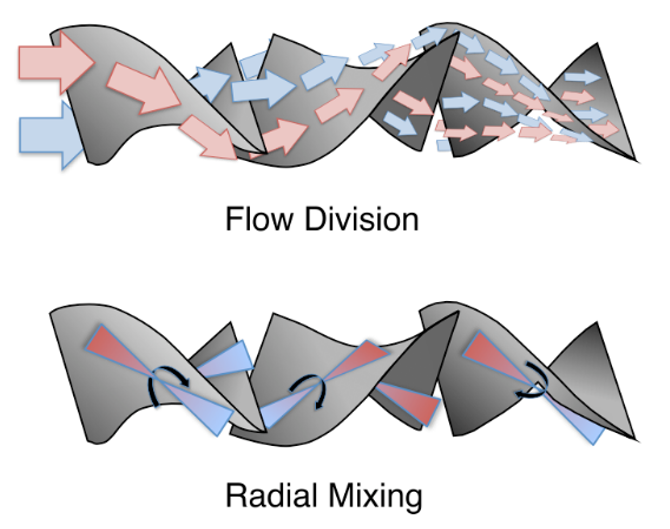
\includegraphics{simulation1.png}}
    \caption{Schéma montrant comment ce mélange un fluide}
    \label{fig:simulation1}
\end{figure}
Une première étape de conception fus donc d'essayer de comprendre à quoi pourrais bien ressembler ce type de mélangeur en 2D.
On sait de par la mécanique des fluides que la pression et la vitesse d'écoulement sont liée à la géométrie du milieu d'écoulement.
Ainsi J'ai modélisé quatre différents mélangeurs afin d'observer le comportement du fluide lors d'une simulation.
De plus le mode de fabrication le plus simple étant la découpe LASER il a fallu adapter la forme de ceux-ci afin qu'il soit réalisable en entier à la découpeuse LASER du campus.
\begin{figure}[H]
    \centering
    \resizebox{\linewidth}{!}{\includegraphics{CAO\_prototype\_melangeur.png}}
    \caption{CAO du mélangeur avec chicanes}
    \label{fig:CAO_prototype_melangeur}
\end{figure}
Comme on peut le voir dans la figure \ref{fig:CAO_prototype_melangeur} le premier mélangeur était juste composé d'un chemin direct auquel ont été ajouté des chicanes droites.
Le flux de liquide assimiler a de l'eau entre par en dessous et sort par au-dessus, et les conditions de pression sont celle donnée dans la datasheet de la pompe étant donné que le mélangeur sera placer juste derrière la pompe.
\begin{figure}[H]
    \centering
    \resizebox{\linewidth}{!}{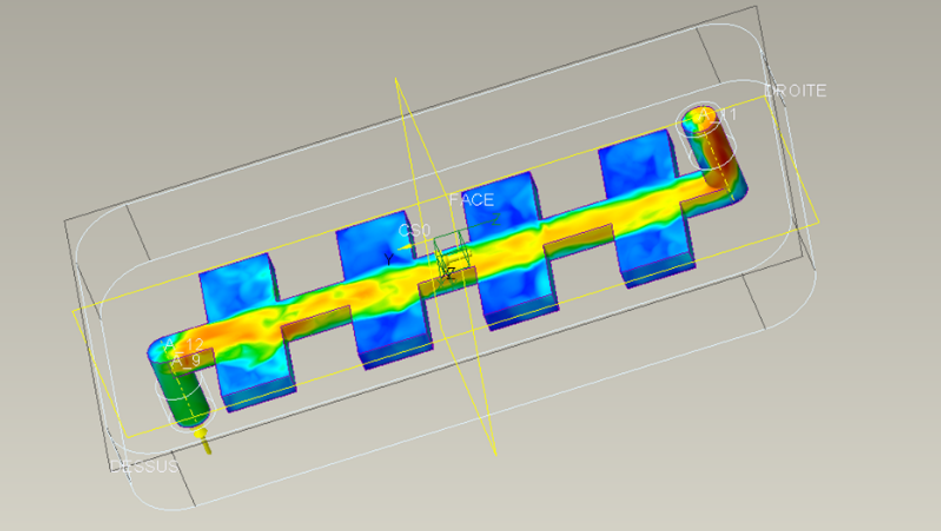
\includegraphics{simulation2.png}}
    \caption{Simulation fluidique du mélangeur à chicanes}
    \label{fig:simulation2}
\end{figure}
Grâce à la figure \ref{fig:simulation2} on peut voir que les chicanes n'apporte pas de plus value pour mélanger le fluide.
\begin{figure}[H]
    \centering
    \resizebox{\linewidth}{!}{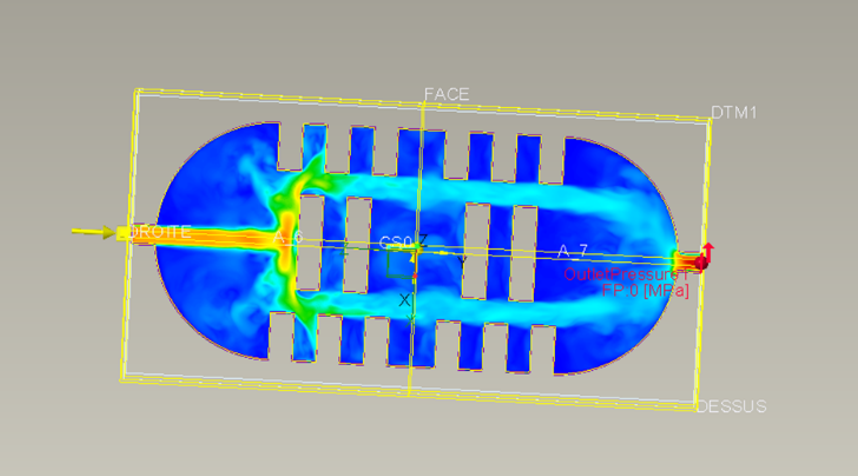
\includegraphics{simulation3.png}}
    \caption{Simulation fluidique avec 2 voies et chicanes}
    \label{fig:simulation3}
\end{figure}
En divisant le flux en deux et en réduisant l'espace des chicanes ont remarque qu'il n'y a que peu d'effet.
Toutefois la division du flux en deux apporte des turbulences lorsque les deux flux se recombinent ainsi que l'obstacle placer perpendiculairement au flux.
\begin{figure}[H]
    \centering
    \resizebox{\linewidth}{!}{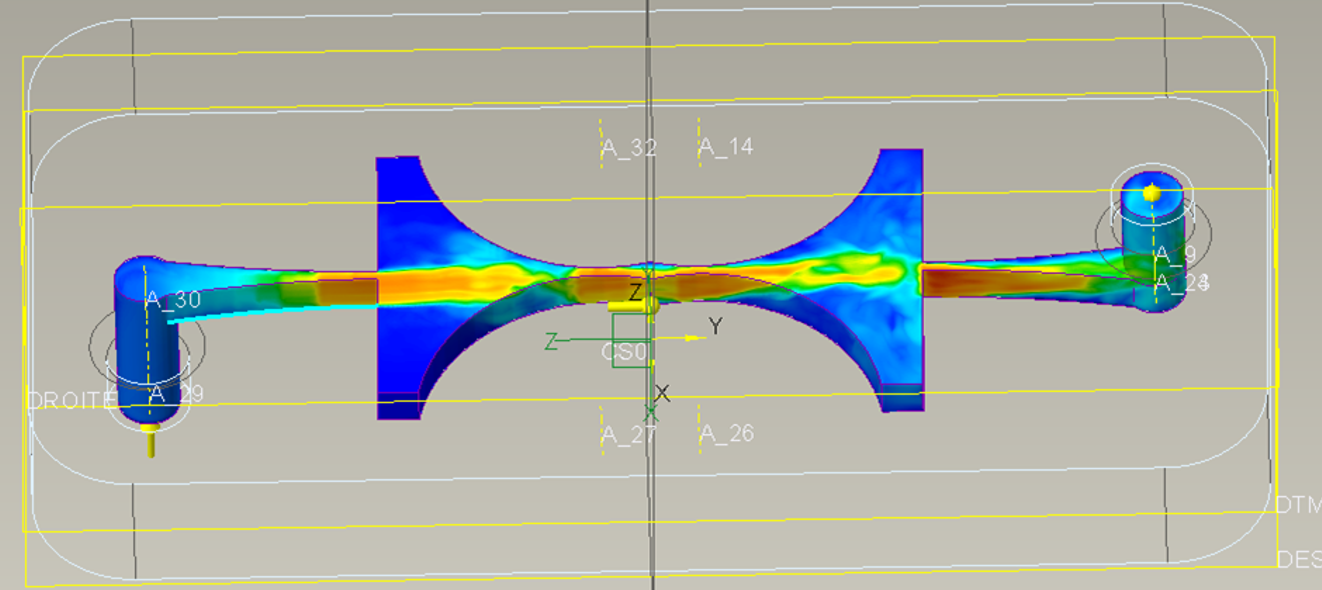
\includegraphics{simulation4.png}}
    \caption{Simulation fluidique avec accélération}
    \label{fig:simulation4}
\end{figure}
Une autre version avait pour idée de détendre et de comprimé le flux afin de crée des turbulences, on voit (zone coloré) que la vitesse augmente mais reste toujours dans le sens du circuit.
Il manque une forme pour casser ce flux.
\begin{figure}[H]
    \centering
    \resizebox{\linewidth}{!}{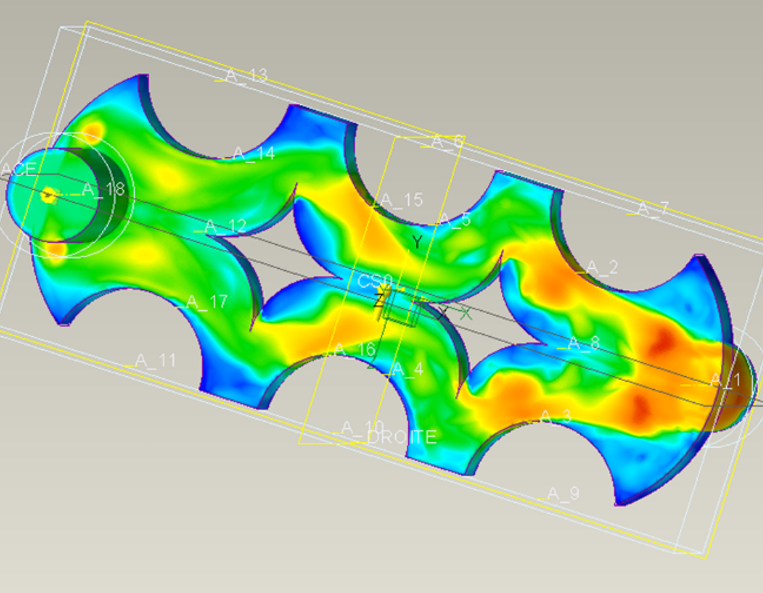
\includegraphics{simulation5.png}}
    \caption{Simulation fluidique avec chicanes et obstacles}
    \label{fig:simulation5}
\end{figure}
Lorsque l'on casse le flux et qu'on le dirige vers un obstacle cela crée des turbulences.
Ce que l'on observe ici c'est une accélération du fluide couplé à des zone de dépression.
Cela cause des turbulences derrière les obstacles placer au centre.
\subsubsection{CAO du mélangeur}
Nous avons donc choisi de partir sur un mélangeur composé de deux parties, l'une central permet de casser de flux et de le séparer en deux.
La partie externe est mobilisé afin de crée des zones d'accélération et de décélération.
\begin{figure}[H]
    \centering
    \resizebox{\linewidth}{!}{\includegraphics{CAO\_melangeur\_couche2.png}}
    \caption{Couche central du mélangeur}
    \label{fig:CAO_melangeur_couche2}
\end{figure}
Notre conception est basée sur un principe de sandwich, une première épaisseur permettant l'étanchéité, le support et le guidage des autres couches.
Une couche centrale munit d'un détrompeur composer d'un élément externe guider par deux goupilles extérieures, et un élément interne guidé par les goupilles intérieures.
Et enfin une dernière couche permettant de fermer le tout, toujours guider par les deux goupilles externes.
L'adhésion et l'étanchéité sera assuré par une couche adhésive déposer sur les plaques.
\begin{figure}[H]
    \centering
    \resizebox{\linewidth}{!}{\includegraphics{CAO\_melangeur.png}}
    \caption{Mélangeur hydrostatique}
    \label{fig:CAO_melangeur}
\end{figure}
\subsection{Zone de culture}
\begin{figure}[H]
    \centering
    \resizebox{\linewidth}{!}{\includegraphics{CAO\_cellule.png}}
    \caption{bio-chip pour les cellules}
    \label{fig:CAO_cellule}
\end{figure}
Pour le biochip contenant les cellules visibles sur la figure \ref{fig:CAO_cellule}, nous avons choisi d'utiliser l'assemblage en plusieurs couches de PMMA.
Celui-ci contient 4 couches d'épaisseur différentes pour répondre à certaines contraintes.
Nous utiliserons des goupilles, pour être sûr que les différents éléments soient bien alignés.
\begin{multicols}{2}
    \begin{figure}[H]
        \centering
        \resizebox{\linewidth}{!}{\includegraphics{CAO\_cellule\_couche1.png}}
        \caption{CAO de la première couche}
        \label{fig:CAO_cellule_couche1}
    \end{figure}
    \begin{figure}[H]
        \centering
        \resizebox{\linewidth}{!}{\includegraphics{CAO\_cellule\_couche2.png}}
        \caption{CAO de la seconde couche}
        \label{fig:CAO_cellule_couche2}
    \end{figure}
\end{multicols}
La couche du dessous fait 0.3 mm d'épaisseur pour permettre l'observation des cellules au microscope.
La 2e couche est prévu pour contenir les cellules mais sera supprimer car elle crée des angles droits qui risque d'endommager les cellules.
\begin{multicols}{2}
    \begin{figure}[H]
        \centering
        \resizebox{\linewidth}{!}{\includegraphics{CAO\_cellule\_couche3.png}}
        \caption{CAO de la troisième couche}
        \label{fig:CAO_cellule_couche3}
    \end{figure}
    \begin{figure}[H]
        \centering
        \resizebox{\linewidth}{!}{\includegraphics{CAO\_cellule\_couche4.png}}
        \caption{CAO de la quatrième couche}
        \label{fig:CAO_cellule_couche4}
    \end{figure}
\end{multicols}
La 3e couche permet au fluide contenant les hormones et nutriment de circuler la où seront accroché les cellules.
L'entrée du fluide est plus étroite que la sortie pour éviter des problèmes de surpression.
Et enfin la dernière couche contient les trous pour chasser les connecteur Luer lock, permettant de relier le bio chip contenant les cellules au reste du système par l'intermédiaire de tuyaux.
Les angles devront être arrondit pour éviter d'endommager les cellules.
\subsection{Support des réservoirs}
\begin{multicols}{2}
    \begin{figure}[H]
        \centering
        \resizebox{\linewidth}{!}{\includegraphics{CAO\_reservoir1.png}}
        \caption{CAO du porte réservoir version 1}
        \label{fig:CAO_reservoir1}
    \end{figure}
    \begin{figure}[H]
        \centering
        \resizebox{\linewidth}{!}{\includegraphics{CAO\_reservoir2.png}}
        \caption{CAO du porte réservoir version 2}
        \label{fig:CAO_reservoir2}
    \end{figure}
\end{multicols}
Désormais nous avons une idée très claire du rendu physique du projet, celui-ci sera composer d'un boitier auxquelles sera fixé les trois pompe, les quatre tube comprenant les hormones, le liquide de culture neuf, et usagé.
Ce boitier sera lui aussi découper au LASER et au besoin renforcé par des pièces imprimé en 3D.
Il ne contiendra pas l'électronique, celui-ci sera placer en dehors de l'incubateur et relier au système via un câble.
Il est à noter qu'il manque les électrovannes, qui ont été modéliser et qui seront placer de l'autre côté des pompes.
\begin{figure}[H]
    \centering
    \resizebox{\linewidth}{!}{\includegraphics{CAO\_electrovanne.png}}
    \caption{CAO des électrovannes}
    \label{fig:CAO_electrovanne}
\end{figure}
\subsubsection{Le boitier découpable au LASER a $ CO_2 $}
A des fin de cout et de rapidité, nous avons fait le choix de fabriquer notre boitier avec le
plus de partie découper au LASER. Pour cela nous avons modéliser chaque face du boitier et nous
les avons fait s'emboiter dans un assemblage.
Pour des questions de maintient, nous avons conçu 8 petites équerres de maintient à visser
et les plaques serons collées entre elles par de la colle à plexiglass.
\begin{figure}[H]
    \centering
    \resizebox{\linewidth}{!}{\includegraphics{CAO\_boitier\_decoupe\_LASER.png}}
    \caption{CAO du boitier à découper au LASER}
    \label{fig:CAO_boitier_decoupe_LASER}
\end{figure}
Nous avons aussi ajouter deux support à imprimer en 3D pour fixer le melangeur et la zone de culture.
\newpage
\subsection{Assemblage des biochips}
Pour réaliser l’assemblage du mélangeur et du biochip qui contiendra les cellules,
la première étapes a été de découper chaque éléments dans des plaques de PMMA.
Afin de facilité l’assemblage, seul la couche du milieu est recouverte de colle
sur ces deux faces. La deuxième étape consiste à assembler le tout.
Les goupilles du gabarit (voir figure \ref{fig:gabarit}) permettent l’alignement
des 3 différentes couches. Une fois les 3 couches superposer,
il faut s’assurer que celle-ci sont correctement collé entre elles.
Pour cela, les trois couches sont pressé entre elles à l’aide d’un rouleau.
Enfin, les luer-lock sont emboiter dans le boichip avec de la colle époxy.
\begin{multicols}{3}
    \begin{figure}[H]
        \centering
        \resizebox{\linewidth}{!}{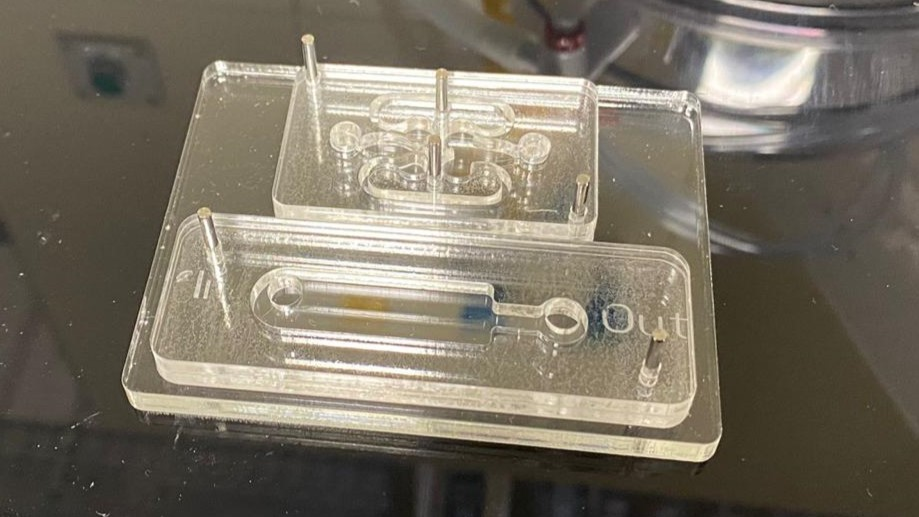
\includegraphics{gabarit.JPG}}
        \caption{Photo du gabarit et des biochips}
        \label{fig:gabarit}
    \end{figure}
    \begin{figure}[H]
        \centering
        \resizebox{\linewidth}{!}{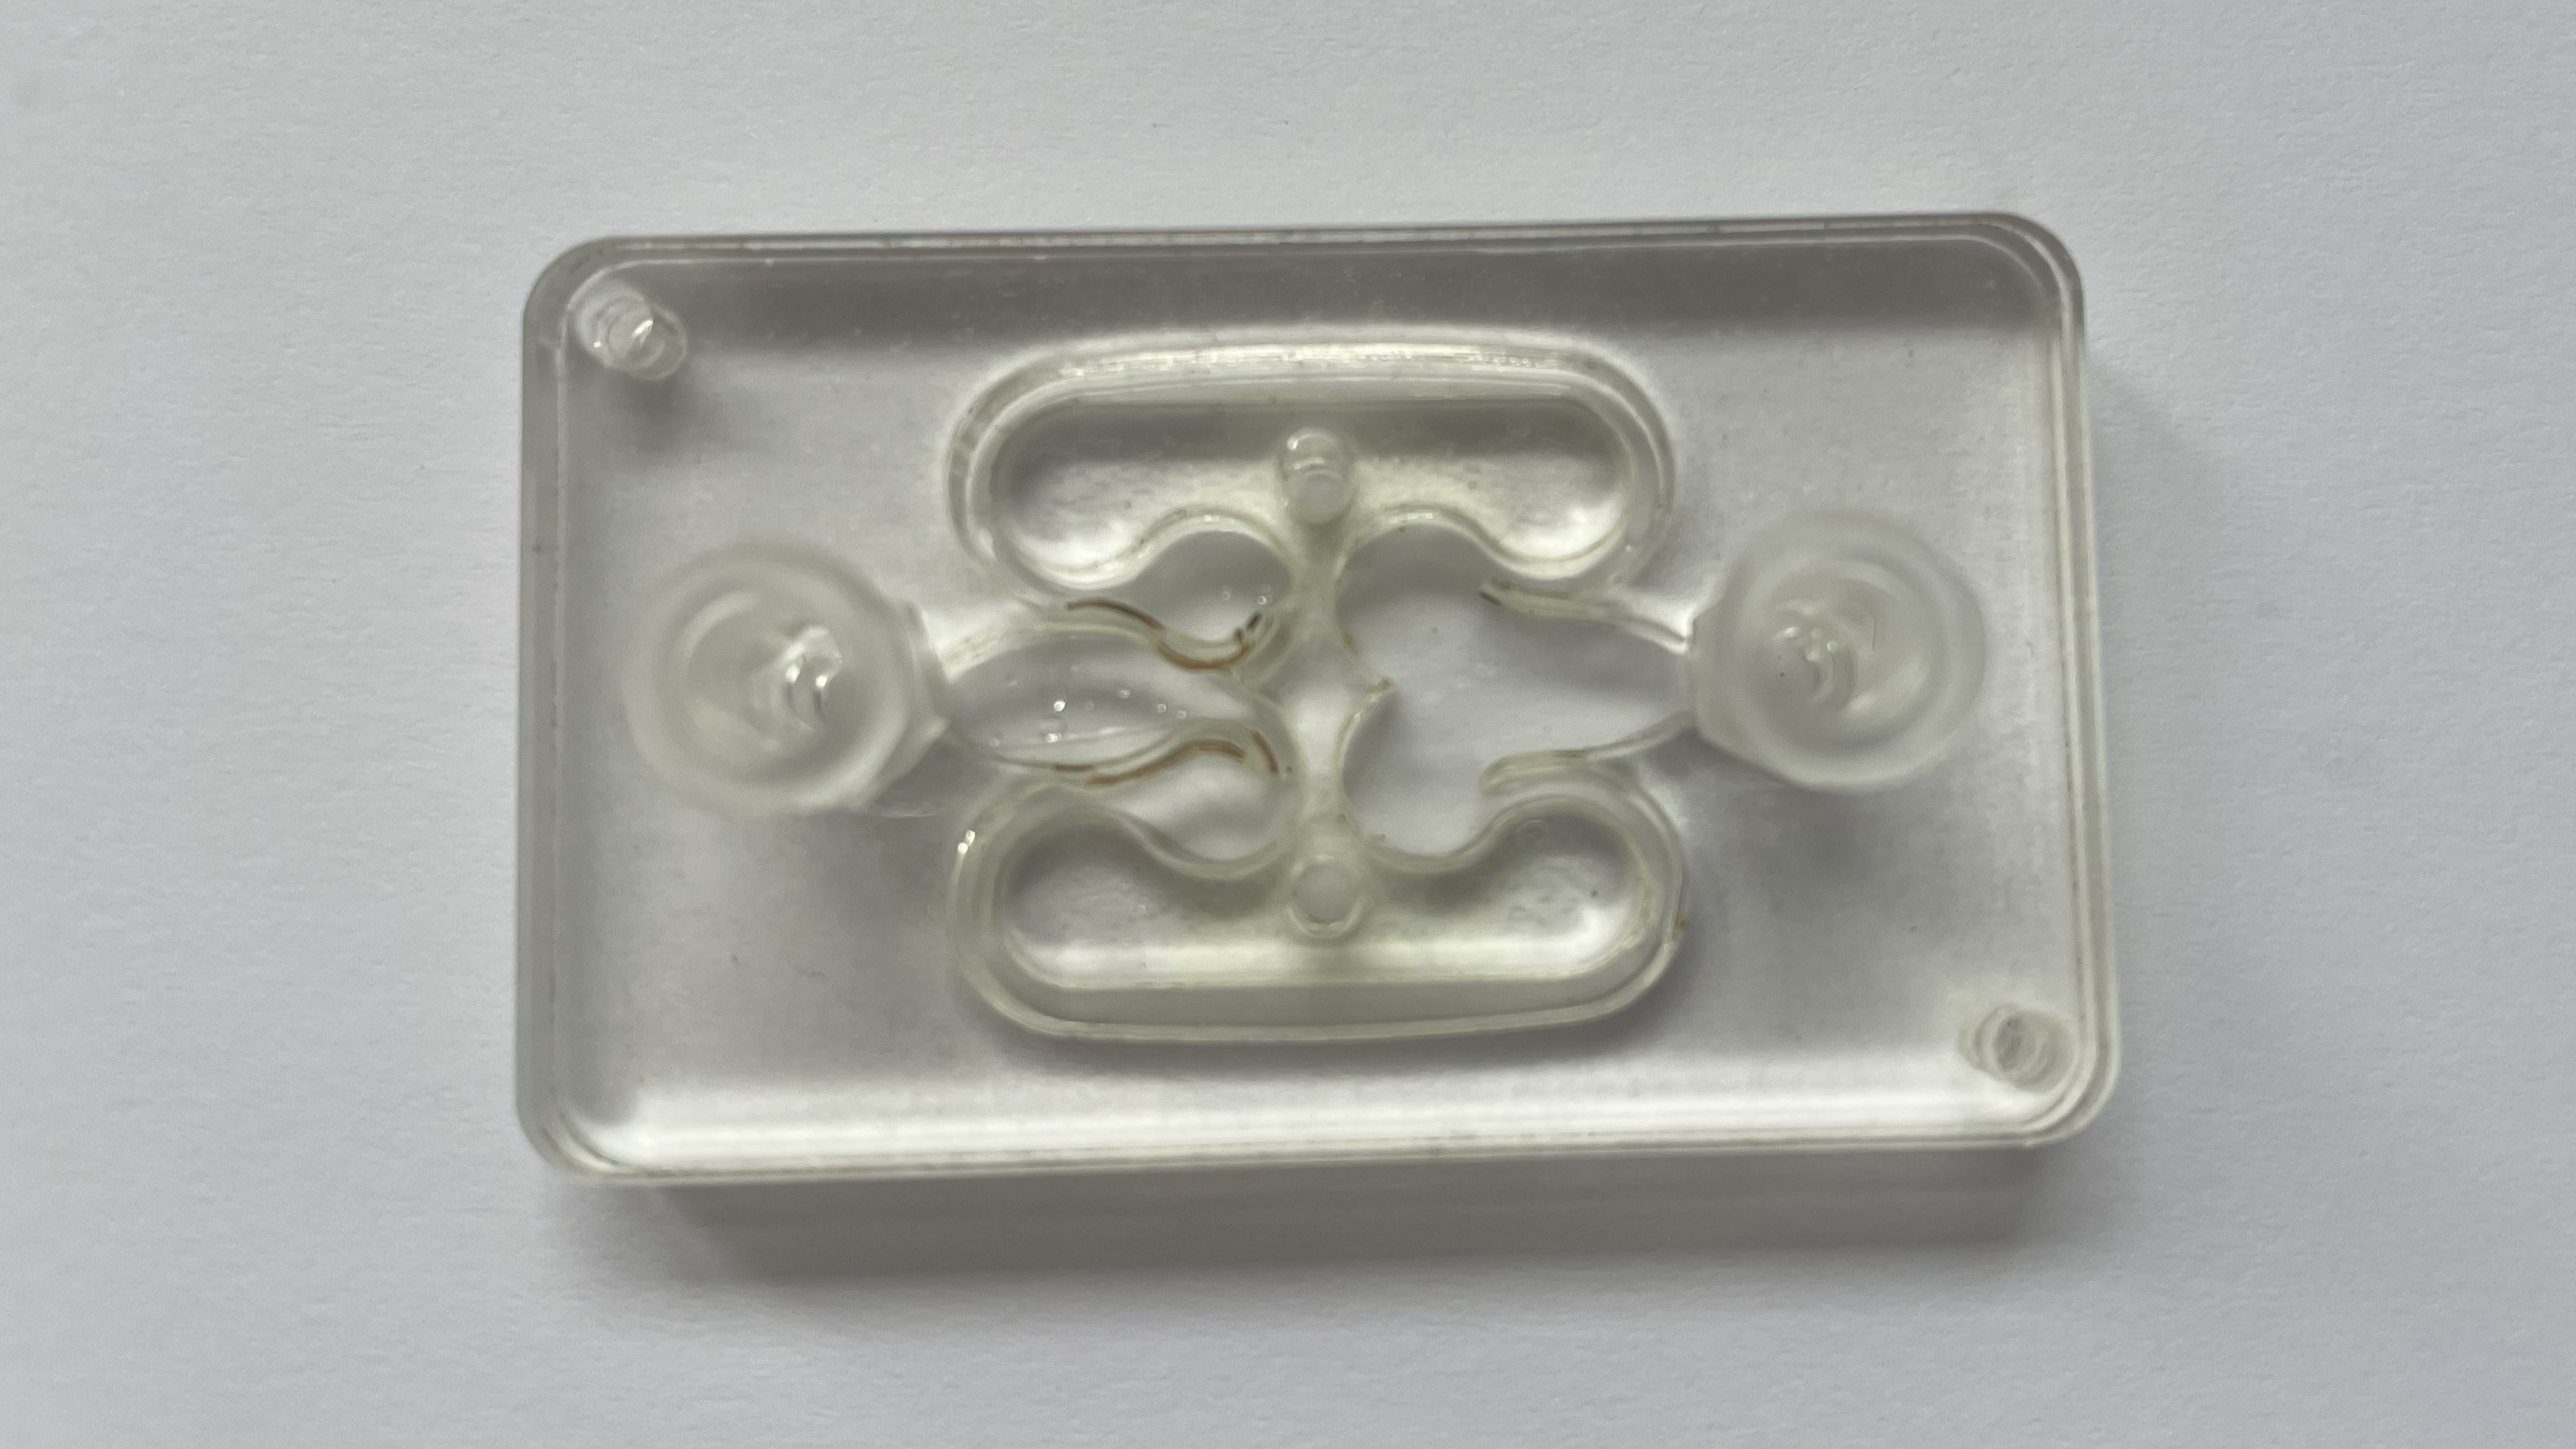
\includegraphics{melangeur.jpg}}
        \caption{Photo de l'assembage du mélangeur}
        \label{fig:melangeur}
    \end{figure}
    \begin{figure}[H]
        \centering
        \resizebox{\linewidth}{!}{\includegraphics{biochip\_cellulesV1.jpg}}
        \caption{Photo de l'assembage du biochip cellules}
        \label{fig:cellules}
    \end{figure}
\end{multicols}
\subsubsection{Le biochip cellules}
\begin{multicols}{2}
    \begin{figure}[H]
        \centering
        \resizebox{\linewidth}{!}{\includegraphics{fluide\_cellulesV1.jpg}}
        \caption{Photo du test fluidique}
        \label{fig: fluide_cellules}
    \end{figure}
    \begin{figure}[H]
        \centering
        \resizebox{\linewidth}{!}{\includegraphics{reste\_fluide\_cellulesV1.jpg}}
        \caption{Photo des restes de liquide}
        \label{fig:reste_cellules}
    \end{figure}
\end{multicols}
Après avoir injecté du fluide dans le biochip, celui-ci ne fuit pas. Cependant, le test a montré une mauvaise optimisation de l'espace. En effet, comme le montre la photo de la figure 4, le liquide reste bloqué à certains endroits. Pour optimiser la circulation du fluide, une nouvelle version de ce biochip a été modélisée.
\newpage
\subsubsection{Modelisation biochip cellules version 2}
\begin{multicols}{2}
    \begin{figure}[H]
        \centering
        \resizebox{\linewidth}{!}{\includegraphics{CAO\_cellulesV2.png}}
        \caption{CAO assemblage biochip cellules V2}
        \label{fig: CAO_cellulesV2}
    \end{figure}
    \begin{figure}[H]
        \centering
        \resizebox{\linewidth}{!}{\includegraphics{CAO\_cellules\_milieu\_V2.png}}
        \caption{CAO milieu du biochip cellules V2}
        \label{fig:milieu_cellulesV2}
    \end{figure}
\end{multicols}
Les entrées et sorties du fluide ont le même diamètre que les trous pour insérer les embouts luer-lock, afin d'éviter d'avoir une zone inutile autour de ces embouts.
De plus, pour la zone plus large qui accueillera les cellules, les angles à 90° ont été remplacés par des angles à 45°. Cela devrait permettre au fluide de mieux circuler dans cette zone.
\subsubsection{Le mélangeur}
Nous avons efectuer les premier tests du mélangeur en faisant circuler du liquide à l'intérieur
a l'aide de seringues.
\begin{figure}[H]
    \centering
    \resizebox{\linewidth}{!}{\includegraphics{fuite\_melangeur.PNG}}
    \caption{Photo test fluidique mélangeur}
    \label{fig:fuite_melangeurV1}
\end{figure}
Comme on peut observer sur la \label{fig:fuite_melangeur} le liquide s'infiltre dans l'intercouche ce qui cause une fuite
par un trou de fabrication.
\subsubsection{CAO mélangeur version 2}
Le premier mélangeur fuyais, cela etait probablement du à une surpression qui causait
l'infiltration du liquide dans l'intercouche.
Le temps nous manque, il nous faut un mélangeur fonctionnel même si il est moins performant que l'ancien.
Nous avons donc conçu une version plus simple et plus robuste qu'il nous reste à tester.
\begin{multicols}{2}
    \begin{figure}[H]
        \centering
        \resizebox{\linewidth}{!}{\includegraphics{CAO\_melangeur\_V2\_couche1.png}}
        \caption{Premiere couche du melangeur V2}
        \label{fig: CAO_melangeur_V2_couche1}
    \end{figure}
    \begin{figure}[H]
        \centering
        \resizebox{\linewidth}{!}{\includegraphics{CAO\_melangeur\_V2\_couche2.png}}
        \caption{Deuxième couche du mélangeur V2}
        \label{fig:CAO_melangeur_V2_couche2}
    \end{figure}
\end{multicols}
Nous avons garder l'idée de séparer puis de refusionner le flux, sauf que le chemin est bien plus simple.
Les dimensions on été agrandi afin d'avoir 1cm de chaque coté ce qui est deux fois plus que l'ancien.
\begin{multicols}{2}
    \begin{figure}[H]
        \centering
        \resizebox{\linewidth}{!}{\includegraphics{CAO\_melangeur\_V2\_couche3.png}}
        \caption{Dernière couche du melangeur V2}
        \label{fig: CAO_melangeur_V2_couche3}
    \end{figure}
    \begin{figure}[H]
        \centering
        \resizebox{\linewidth}{!}{\includegraphics{CAO\_melangeur\_V2.png}}
        \caption{L'assemblage du mélangeur V2}
        \label{fig:CAO_melangeur_V2}
    \end{figure}
\end{multicols}
Nous avons ainsi un nouveau mélangeur de 100 par 50 a placer dans le système. La piece permettant la fixation du mélangeur
au boitier a donc été ajusté.
\subsubsection{CAO boitier version 2}
\begin{figure}[H]
    \centering
    \resizebox{\linewidth}{!}{\includegraphics{CAO\_boitier\_decoupe\_LASER\_V2.png}}
    \caption{Boitier modifier pour accueillir le melangeur V2}
    \label{fig:CAO_boitier_V2}
\end{figure}
Nous obtenons donc ce rendu, il reste alors a le découper et a l'assembler.
\newpage
\section{Conception électronique et programmation}
\subsection{Carte d'alimentation version 1}
\begin{figure}[H]
    \centering
    \resizebox{\linewidth}{!}{\includegraphics{carte\_alimentation.png}}
    \caption{Montage électronique pour l'alimentation du Raspberry Pi et des pompes version 1}
    \label{fig:CAO_electronique_V1}
\end{figure}
L'alimentation de tous le biochip se fera via l'alimentation d'un Arduino de 60 W.
Il arrive sur la carte d'alimentation via la connectique circulaire JAlim.
U1 est un régulateur de tension à découpage de la marque TRACO, il permet de descendre la tension de 12V à 5V il sert à alimenter le Raspberry pi qui sera alimenter par ses pins GPIO.
Les moteurs seront contrôlés par les mosfet M1, M2 et M3.
Les moteurs seront branchés à la carte via des connecteurs circulaire afin que le système soit le plus flexible possible.
Les diodes D1, D2 et D3 sont des diodes de roues libres.
\newpage
\subsubsection{Carte d'alimentation version 2 et 3}
Lorsque nous avons testé la première version du circuit électronique nous avons remarqué que le montage ne fonctionnait pas.
En effet nous avons remarqué que le raspberry pi ne fournit pas assez de tension aux mosfets pour alimenter les pompes.
Pour pouvoir alimenter correctement les pompes une tension de 3,5 V est nécessaire à la "gate" des mosfets.
Cependant le raspberry pi ne peut fournir qu'une tension de 3,3 V via les pins qui sont contrôlables.
\begin{figure}[H]
    \centering
    \resizebox{\linewidth}{!}{\includegraphics{carte\_alimentationV2.png}}
    \caption{Montage électronique pour l'alimentation du Raspberry Pi et des pompes version 2}
    \label{fig:CAO_electronique_V2}
\end{figure}
Pour obtenir la tension adéquate nous avons amplifié le signal grâce à un AOP pour pouvoir piloter les pompes.
Les AOP devaient être alimentés via le 12 V du transformateur.
Après plusieurs essais infructueux nous avons remarqué que les AOP que nous avons choisies ne peuvent être alimentées par une alimentation non-symétrique.
En alimentant les amplificateurs via une alimentation de laboratoire stabilisé avec une tension symétrique +5/-5 V le montage fonctionnait correctement.
\begin{figure}[H]
    \centering
    \resizebox{\linewidth}{!}{\includegraphics{carte\_alimentationV3.png}}
    \caption{Montage électronique pour l'alimentation du Raspberry Pi et des pompes version 3}
    \label{fig:CAO_electronique_V3}
\end{figure}
Nous avons récupéré de nouveau amplificateurs qui sont compatibles en alimentation non-symétrique, pour éviter de devoir alimenter une partie du montage via une alimentation de laboratoire.
Comme nous avons reçu les nouveaux amplificateurs assez tardivement, nous n'avons pas eu le temps de tester le montage avec les nouveaux amplificateurs.
Si les amplificateurs ne conviennent pas nous resterons sur l'alimentation de laboratoire pour alimenter les amplificateurs.
\subsection{Programmation}
\subsubsection{GitHub}
On a mis en place un GitHub pour se partager les codes de programmation, le "repo" contient aussi une ébauche du guide d'utilisateur.
Le guide d'utilisateur contient actuellement uniquement les requirements pour le Raspberry pi ainsi que les commandes à utiliser.
\subsubsection{Raspberry Pi}
On a configuré le Raspberry pi 4 pour qu'on puisse se connecter dessus à distance à l'aide du protocole SSH.
On peut s'y connecter facilement dessus à partir du moment que l'on se trouve sur le même réseau wifi.
On peut lui transmettre des fichiers ainsi que récupérer des fichiers qui sont stockées dessus.
\subsubsection{Préparation des données}
Ce code permet de préparer les datas afin de pouvoir être utiliser par le logiciel qui contrôle le biochip.
Il a été conçu pour que l'utilisateur rentre un minimum de donner afin de gagner du temps.
Il permet de convertir un fichier csv que l'utilisateur aura créée au préalable avec les différents jalons de concentration en un fichier qui contient toutes les concentrations de l'expérience sur 28 jours.
Sur la figure \ref{fig:dataPreparation} on peut voir une représentation des données rentrées par l'utilisateur et les données produites par le programme.
\begin{figure}[H]
    \centering
    \resizebox{\linewidth}{!}{\includegraphics{representation\_data\_gen.png}}
    \caption{Données généré par le programme avec les données rentrées par l'utilisateur}
    \label{fig:dataPreparation}
\end{figure}
On peut l'utiliser directement sur un ordinateur puis envoyer le fichier généré sur le Raspberry pi ou bien on peut envoyer le fichier csv sur le Raspberry pi puis le généré directement sur le Raspberry pi.
Le fichier généré est un fichier de type ftr il n'est donc pas lisible directement ceci est fait afin de gagner en rapidité d'exécution et gagner du stockage.
Si on utilisait un fichier csv équivalent il contiendrait tellement de donnés qu'il faudrait plusieurs secondes pour le généré et il prendrait 10 fois plus de stockage.
Le fichier à préparer doit être présenter sous la forme :
\begin{table}[H]
    \centering
    \begin{tabular}{lll}
        Time & Conc1 & Conc2 \\
        0    & 1     & 1     \\
        2    & 6     & 8     \\
        10   & 2     & 1     \\
        15   & 4     & 2
    \end{tabular}
\end{table}
\subsubsection{Programme de test des moteurs}
Nous avons réalisé un code python qui permet de vérifier si le contrôle des moteurs fonctionne bien.
En plus de ça il permet d'effectuer les tests de débits des pompes.
Normalement il faudrait environ 30 minutes pour pouvoir tester les débits de toutes les pompes sur une plage de tension d'alimentation des pompes de 6 V à 12 V.
Le code qui permet de contrôler les pompes sera le même que celui dans le programme principal.
Cela va nous permettre de gagner du temps lors du développement de celui-ci.
\newpage
%\section{Conclusion}
%Pour conclure on peut commencer la découpe du mélangeur et de la zone de culture afin de commencer les tests.
%Nous devons terminer le montage électrique et tester les pompes.
%Si les essais se déroulent comme prévu nous allons pouvoir avancer rapidement sur la programmation et la réalisation d'un prototype fonctionnel.
%\newpage
%\section{Annexe}
%
%\newpage
\printbibliography

\end{document}